\UseRawInputEncoding
\documentclass[a4paper, 14pt]{extarticle}

% Поля
%--------------------------------------
\usepackage{geometry}
\geometry{a4paper,tmargin=2cm,bmargin=2cm,lmargin=3cm,rmargin=1cm}
%--------------------------------------


%Russian-specific packages
%--------------------------------------
\usepackage[T2A]{fontenc}
\usepackage[utf8]{inputenc} 
\usepackage[english, main=russian]{babel}
\usepackage{cmap}
%--------------------------------------

\usepackage{textcomp}

% Красная строка
%--------------------------------------
\usepackage{indentfirst}               
%--------------------------------------             


%Graphics
%--------------------------------------
\usepackage{graphicx}
\graphicspath{ {./images/} }
\usepackage{wrapfig}
%--------------------------------------

% Полуторный интервал
%--------------------------------------
\linespread{1.3}                    
%--------------------------------------

%Выравнивание и переносы
%--------------------------------------
% Избавляемся от переполнений
\sloppy
% Запрещаем разрыв страницы после первой строки абзаца
\clubpenalty=10000
% Запрещаем разрыв страницы после последней строки абзаца
\widowpenalty=10000
%--------------------------------------

%Списки
\usepackage{enumitem}

%Подписи
\usepackage{caption} 

%Гиперссылки
\usepackage{hyperref}

\hypersetup {
	unicode=true
}

%Рисунки
%--------------------------------------
\DeclareCaptionLabelSeparator*{emdash}{~--- }
\captionsetup[figure]{labelsep=emdash,font=onehalfspacing,position=bottom}
%--------------------------------------

\usepackage{tempora}
\usepackage{amsmath}
\usepackage[dvipsnames]{xcolor}
\usepackage{listings}
\lstset{
  belowcaptionskip=1\baselineskip,
  breaklines=true,
  frame=L,
  xleftmargin=\parindent,
  language=Java,
  showstringspaces=false,
  basicstyle=\footnotesize\ttfamily,
  keywordstyle=\bfseries\color{blue},
  commentstyle=\itshape\color{purple},
  identifierstyle=\color{black},
  stringstyle=\color{red},
  numbers=left,           
  numberstyle=\tiny\color{gray}, 
  numbersep=10pt,      
  % ------------------------------
}

%--------------------------------------
%			НАЧАЛО ДОКУМЕНТА
%--------------------------------------

\begin{document}

%--------------------------------------
%			ТИТУЛЬНЫЙ ЛИСТ
%--------------------------------------
\begin{titlepage}
\thispagestyle{empty}
\newpage


%Шапка титульного листа
%--------------------------------------
\vspace*{-60pt}
\hspace{-65pt}
\begin{minipage}{0.3\textwidth}
\hspace*{-20pt}\centering

\includegraphics[width=\textwidth]{emblem}
\end{minipage}
\begin{minipage}{0.67\textwidth}\small \textbf{
\vspace*{-0.7ex}
\hspace*{-6pt}\centerline{Министерство науки и высшего образования Российской Федерации}
\vspace*{-0.7ex}
\centerline{Федеральное государственное бюджетное образовательное учреждение }
\vspace*{-0.7ex}
\centerline{высшего образования}
\vspace*{-0.7ex}
\centerline{<<Московский государственный технический университет}
\vspace*{-0.7ex}
\centerline{имени Н.Э. Баумана}
\vspace*{-0.7ex}
\centerline{(национальный исследовательский университет)>>}
\vspace*{-0.7ex}
\centerline{(МГТУ им. Н.Э. Баумана)}}
\end{minipage}
%--------------------------------------

%Полосы
%--------------------------------------
\vspace{-25pt}
\hspace{-35pt}\rule{\textwidth}{2.3pt}

\vspace*{-20.3pt}
\hspace{-35pt}\rule{\textwidth}{0.4pt}
%--------------------------------------

\vspace{1.5ex}
\hspace{-35pt} \noindent \small ФАКУЛЬТЕТ\hspace{80pt} <<Информатика и системы управления>>

\vspace*{-16pt}
\hspace{47pt}\rule{0.83\textwidth}{0.4pt}

\vspace{0.5ex}
\hspace{-35pt} \noindent \small КАФЕДРА\hspace{50pt} <<Теоретическая информатика и компьютерные технологии>>

\vspace*{-16pt}
\hspace{30pt}\rule{0.866\textwidth}{0.4pt}
  
\vspace{11em}

\begin{center}
\Large {\bf Лабораторная работа № 3} \\ 
\large {\bf по курсу <<Языки и методы программирования>>} \\ 
\large <<Полиморфизм на основе интерфейсов в языке Java>>
\end{center}\normalsize

\vspace{8em}


\begin{flushright}
  {Студент группы ИУ9-21Б Воронков А. С.\hspace*{15pt} \\
  \vspace{2ex}
  Преподаватель Посевин Д. П.\hspace*{15pt}}
\end{flushright}

\bigskip

\vfill
 

\begin{center}
\textsl{Москва 2026}
\end{center}
\end{titlepage}
%--------------------------------------
%		КОНЕЦ ТИТУЛЬНОГО ЛИСТА
%--------------------------------------

\renewcommand{\ttdefault}{pcr}

\setlength{\tabcolsep}{3pt}
\newpage
\setcounter{page}{2}

\section{Цель}\label{Sect::task}
\par 
Приобретение навыков реализации интерфейсов для обеспечения возможности 
полиморфной обработки объектов класса 
\section{Задание}
Требуется разработать на языке Java класс с реализованным интерфейсом Comparable<T>
Класс квадратных целочисленных матриц размера n с порядком на основе 
количества элементов, нарушающих симметричность матрицы относительно 
главной диагонали. 
\pagebreak
\section{Практическая реализация}
Код файла Matrix.java
\begin{lstlisting}
package lab3;

public class Matrix implements Comparable<Matrix>{
    public int n;
    private int[][] mat;

    public Matrix(int n) {
        this.n = n;
        mat = new int[n][n];
    }

    public void repl(int i, int j, int x) {
        mat[i][j] = x;
    }

    public int cntAntisim() {
        int cnt = 0;
        for (int i = 0; i < n; i++) {
            for (int j = i; j < n; j++) {
                cnt += (mat[i][j] != mat[j][i]) ? 1 : 0;
            }
        }
        return cnt;
    }

    public int compareTo(Matrix obj) {
        int a_cnt = this.cntAntisim();
        int b_cnt = obj.cntAntisim();
        if (a_cnt > b_cnt) {
            return 1;
        } else if (a_cnt < b_cnt) {
            return -1;
        }
        return 0;
    }

    public String toString() {
        int mx = 0;
        for (int i = 0; i < n; i++) {
            for (int j = 0; j < n; j++) {
                mx = Math.max(mx, String.valueOf(mat[i][j]).length());
            }
        }

        StringBuilder s = new StringBuilder();
        for (int i = 0; i < n; i++) {
            s.append("[ ");
            for (int j = 0; j < n; j++) {
                s.append(String.format("%" + (mx + 1) + "d ", mat[i][j]));
            }
            s.append("]\n");
        }
        return s.toString();
    }
}
\end{lstlisting}
\per
Код файла Test.java
\begin{lstlisting}
package lab3;

import java.util.Arrays;

public class Test {
    public static void main(String[] args) {
        Matrix mt1 = new Matrix(5);
        for (int i = 0; i < mt1.n; i++) {
            for (int j = 0; j < mt1.n; j++) {
                mt1.repl(i, j, i + j);
            }
        }

        int x = 0;
        Matrix mt2 = new Matrix(5);
        for (int i = 0; i < mt2.n; i++) {
            for (int j = 0; j < mt2.n; j++) {
                mt2.repl(i, j, x);
                x++;
            }
        }

        Matrix mt3 = new Matrix(4);
        for (int i = 0; i < mt3.n; i++) {
            for (int j = 0; j < mt3.n; j++) {
                mt3.repl(i, j, i - j);
            }
        }

        Matrix[] mats = new Matrix[] {mt1, mt2, mt3};
        System.out.println("Before sort");
        for (Matrix m : mats) {
            System.out.println(m);
        }
        Arrays.sort(mats);
        System.out.println("After sort");
        for (Matrix m : mats) {
            System.out.println(m);
        }
    }
}
\end{lstlisting}

\section{Результаты}
В результате лабораторной работы был создан класс матриц и для него определен метод сравнения при сортирвке

\begin{center}
    \nopagebreak
    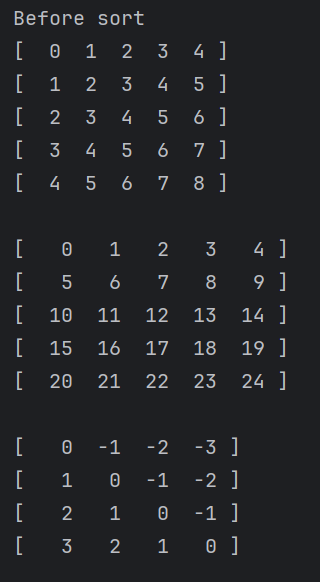
\includegraphics[width=0.85\textwidth]{lab3_1}
    \captionsetup{justification=centering}

    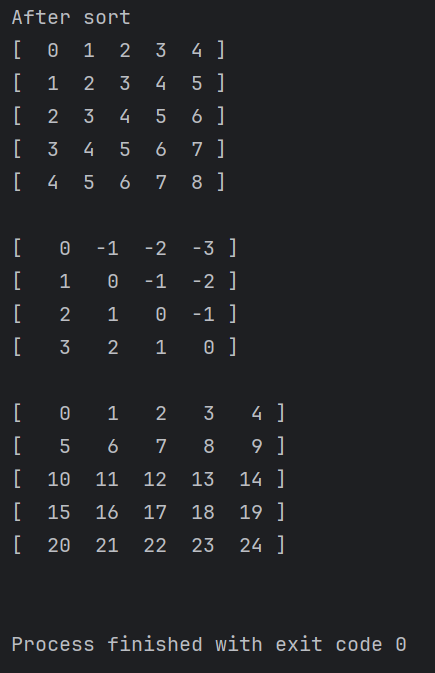
\includegraphics[width=0.85\textwidth]{lab3_2}
    \captionsetup{justification=centering}
    \captionof{figure}{Результат работы Main.java}
\end{center}

\section{Вывод}
В данной лабораторной работе были получены навыки работы с интерфейсами
\end{document}